\section{Trust in social networks}

Users form a social circle because of trust, and through socialization, trust is 
continuously renewed and strengthened. Once trust is established, the social relationship 
between users is gradually transmitted and reproduced\cite{b25, b27}. Therefore, trust is crucial in 
social networks, and it is the foundation of socialization\cite{b28}. The key to the study of 
trust-based recommendation algorithms in social networks lies in the mining and utilization 
of trust information, so we first introduce the concept of trust.

\subsection{Definition and nature of trust}
Trust is a complex concept, which has different understandings and definitions depending 
on the research scope. In computer science, trust denotes contracts and commitments 
based on objects such as identity certificates, passwords, and cryptosystems\cite{b29}. From the 
field of recommender systems, Golbeck defines trust as\cite{b18}: assuming that the behavior of user 
$B$ will bring favorable references and better results to user $A$, then $A$ can be assumed 
to trust $B$~\cite{b26}. The following Figure Trust network is an example 
of a trust network, $1 - 6$ these 6 nodes represent users, the edge between the nodes for the 
trust relationship, the weight on the edge represents the value of the degree of trust, such 
as user 1 pointing to the edge of user 4 has a weight of 0.4, indicating that the degree of 
trust of user 1 on the user 4, indicating that the trust degree of user 1 to user 4 is 0.4\cite{b15}.

\begin{figure}[H] %H为当前位置,!htb为忽略美学标准,htbp为浮动图形
    \centering %图片居中
    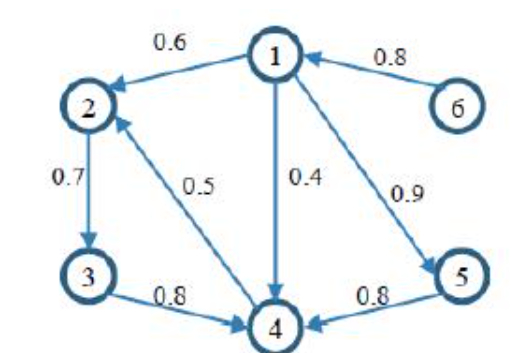
\includegraphics[width=0.4\textwidth]{figures/weight.png} %插入图片,[]中设置图片大小,{}中是图片文件名
    \caption{Trust network} %最终文档中希望显示的图片标题
    \label{Fig.2: Trust network} %用于文内引用的标签
    \end{figure}
\\
Trust is a complex network relationship, characterized by difference, ambiguity, 
transmission, asymmetry, combination, dynamics and so on, described as follows\cite{b15, b18}.

1.
\textbf{Difference}:
trust is a kind of subjective judgment, affected by the objective environment, but 
determined by the subject's own situation, different users for the trust of the judgment 
standard is not uniform\cite{b15}.

2.
\textbf{Ambiguity}:
the size of trust can be expressed and calculated numerically, but trust itself has 
uncertainty, i.e., it is impossible to define the marginal value of trust or distrust\cite{b15}.

3.
\textbf{Transferability}:
trust can be transferred, as shown in the Figure \ref{Fig.2: Transitive properties of trust}
, assuming that user $A$ has 
trust in $B$ and user $B$ has trust in $C$, then we can determine that $A$ also trusts 
$C$ to a certain extent\cite{b15}.

\begin{figure}[H] %H为当前位置,!htb为忽略美学标准,htbp为浮动图形
    \centering %图片居中
    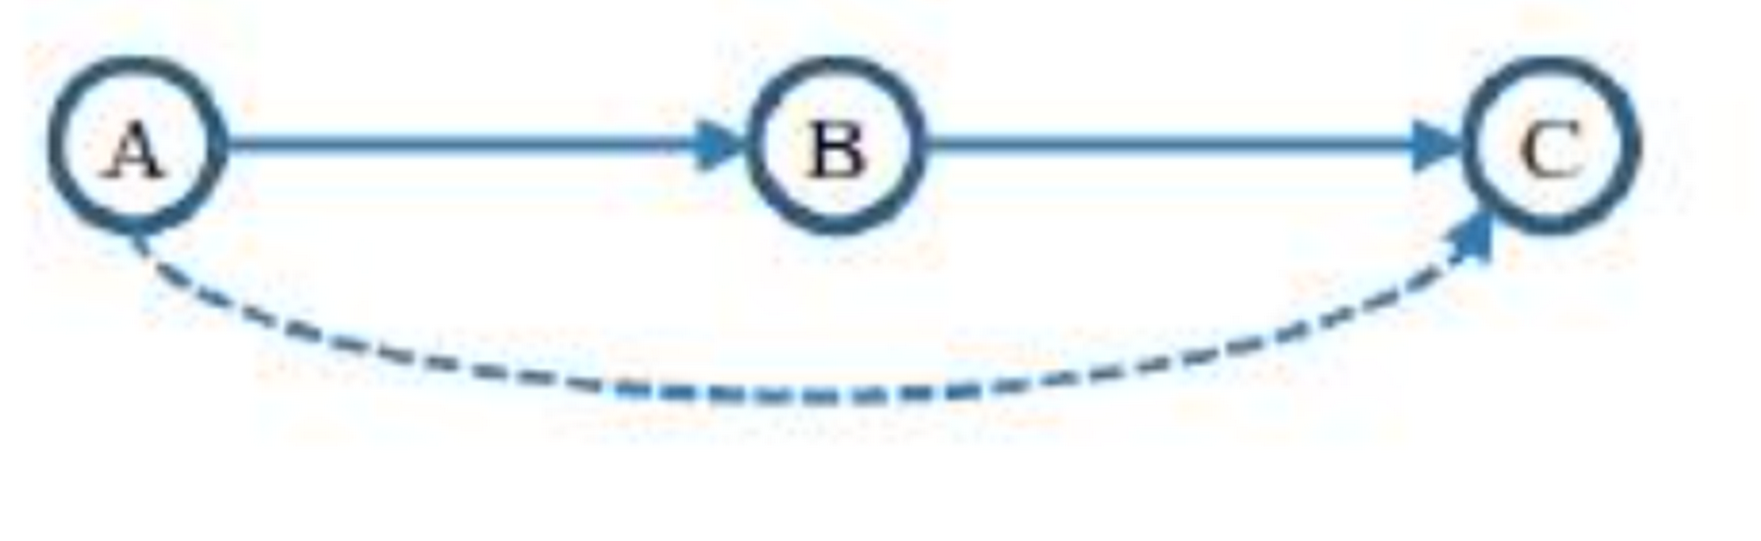
\includegraphics[width=0.4\textwidth]{figures/relation.png} %插入图片,[]中设置图片大小,{}中是图片文件名
    \caption{Transitive properties of trust} %最终文档中希望显示的图片标题
    \label{Fig.2: Transitive properties of trust} %用于文内引用的标签
    \end{figure}
\\

4.
\textbf{Asymmetry}:
the trust relationship is directional, the fact that a user $A$ trusts $B$ does not mean 
that the opposite is also true\cite{b15}.

5.
\textbf{Combinatorial}:
two users who are not adjacent to each other can calculate the indirect trust through 
the intermediate transfer path. The combination can vary depending on the algorithm\cite{b15}.

6.
\textbf{Dynamic}:
Trust is not fixed once it is established, but can change and be updated at any time. 
Influencing factors include the passage of time, the acquisition of domain knowledge, 
changes in the objective environment, and the enhancement of competence\cite{b15}.

\subsection{Categorization and measurement of trust}
Trust is categorized and measured in different ways.
\\
There are different classifications of trust and variations in measurement methods\cite{b28, b29}. 
Trust can be categorized in three different ways, including pairwise and groupwise, 
centralized and distributed, and global and local. Among them, global and local approaches 
are the most popular classification methods, i.e., the global trust degree of each user 
node in the whole network and the local trust degree of friends.

1.
\textbf{Global trust}:
also called reputation, indicates that a user's trust in the social network is referenced 
to the combined evaluation of all other nodes\cite{b22}. Generally, two methods are used 
to calculate the global trust degree, namely, statistical method and iterative method: 
statistical method records the number of trust or distrust, which is expressed by simple 
formula such as ratio; iterative method such as PageRank, EigenTrust, etc\cite{b15}.

2.
\textbf{Local trust}:
it represents one-to-one trust between two users, independent of other users' opinions 
and attitudes towards the target user, and can be categorized into direct and indirect 
trust according to whether a direct connection is established or not\cite{b15}.

\\
Compared with global trust, the research ideas and methods of local trust are various and 
relatively more complicated. Therefore, the weighted trust is introduced.
\\
\textbf{Trust-based weighting}:
The value of user $A$'s preference for an item is the average of the ratings of 
all users $U$ who are familiar with the user $B$. A recommendation strategy that 
uses this approach as a baseline is called trust-based weighted averaging\cite{b15}.
\\
By width-first searching all the paths that can reach the target node from the start node, 
and filtering out the set of users with the maximum trust between the target node and 
the set of users, take a weighted average of the way to consider all the users in the 
set of the target node trust, and constantly iterative update\cite{b27}.
\\
There is also an algorithm based on trust collaborative filtering. In the collaborative 
filtering algorithm, the rating of user $A$ on item $I$ is assumed to be unknown, then it 
can be obtained by referring to the historical behavior of user $A$'s neighbors through 
their explicit ratings for item $I$\cite{b29}.
\\
Collaborative filtering algorithm is based on the improvement of the weighting algorithm, 
both have many common points, such as the use of trust propagation attribute, the 
calculation of the trust degree are used in the way of weighted average\cite{b15}. But there are 
also differences between the two, collaborative filtering algorithm of the maximum path 
threshold is set in advance, the entire search process is static; while the weighted 
algorithm of the maximum propagation distance with different users can make corresponding 
adjustments and appropriate changes. In addition, when predicting trust scores, the latter 
uses collaborative filtering, while the former still uses the weighted average method\cite{b27}.

\subsection{Calculation of trust and similarity}
Global trustworthiness is more commonly known as prestige, reputation, influence, etc. in 
daily life, which indicates the reliability of a user in the whole social network and is 
determined by the user's own qualities such as honesty and competence\cite{b25}. In addition, the 
value of user's trust to other users is weighted,differentiated according to the global 
trust of the trusted person and the subjective trust of the trustor,and the effects of both 
are taken into account in a comprehensive way,while the propagation characteristic of trust 
is introduced to calculate the user-to-user trust\cite{b26}.

In future research, we need to pay attention to the calculation of similarity. 
There are many methods to calculate similarity,the simplest is Euclidean distance,
other common methods are correlation similarity(Pearson correlation coefficient),
cosine similarity and modified cosine similarity\cite{b15}.